La première partie du projet consiste à installer ARGoS, guider un robot à un point donné et remplir l'objectif lorsque les robots sont omniscients comme le présente le cahier des charges \cite{cahierCharges}. Celle-ci a, en effet, été achevée. L'installation a été réalisée avec succès par tous les membres du groupe. Les robots parviennent aux points désignés tout en évitant les obstacles. De plus, ils peuvent, étant omniscients, faire des allers-retours entre le source et le nid. Les robots ont aussi la faculté de détecter une source grâce à ses senseurs et de tenir compte de l'épuisement de leur batterie. Ceci est illustré sur la figure \ref{fig:ourArgos}. Dans le cas de la figure \ref{fig:argosNest}, on  peut observer les robots qui se dirigent vers la source. Sur l'autre figure, les robots sont  de retour au nid.

\begin{figure}[h!]
        \centering
        \begin{subfigure}[h!]{0.4\textwidth}
                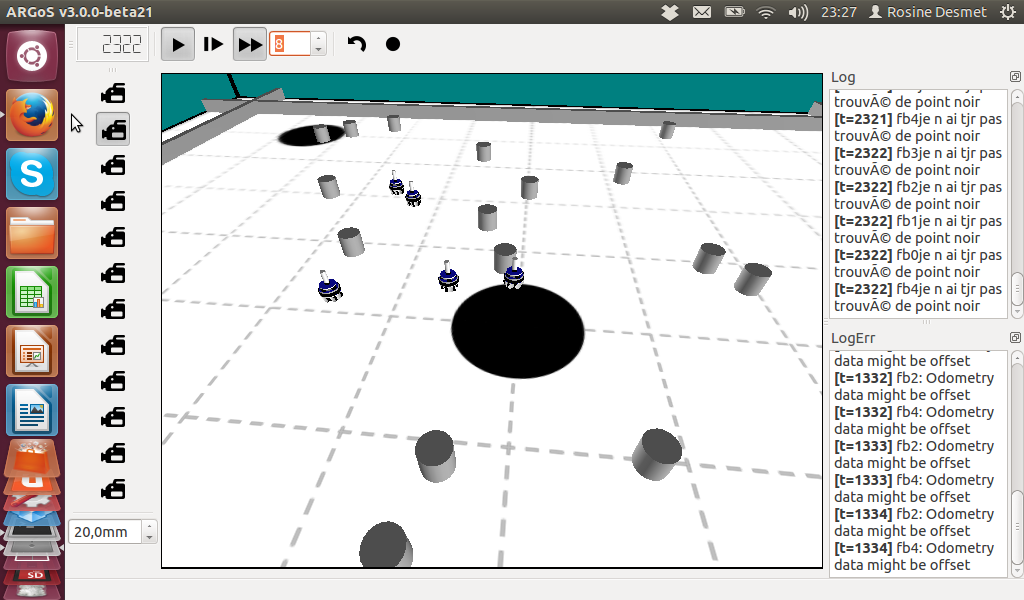
\includegraphics[trim = 60mm 40mm 75mm 45mm, clip, width=\textwidth]{pics/ourArgos1.png}
                \caption{footbots allant à la source}
        \end{subfigure}   \begin{subfigure}[h!]{0.4\textwidth}
                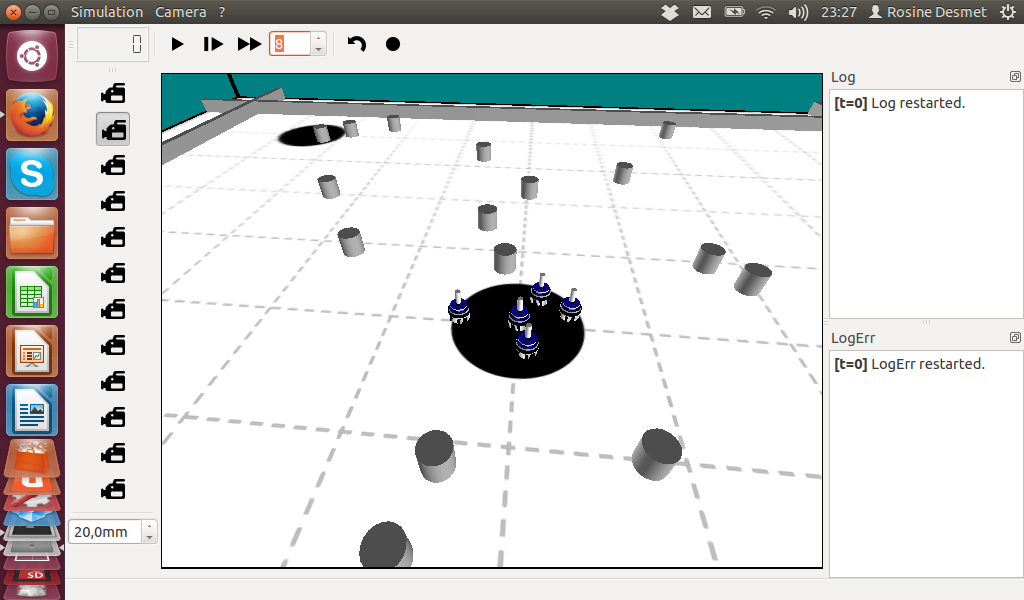
\includegraphics[trim = 60mm 40mm 75mm 45mm, clip, width=\textwidth]{pics/ourArgos2.png}
                \caption{footbots dans le nid\label{fig:argosNest}}
        \end{subfigure}
        \caption{Exécution d'ARGoS avec le comportement produit\label{fig:ourArgos}}
\end{figure}

La création d'une collaboration au sein de l'essaim, le choix et l'intégration d'une communication entre robots, font partie de la seconde partie du projet. A ce niveau, grâce à une études des déplacements de base, la non-omniscience des robots peut déjà être gérée et des recherches sur la communication entre robots ont déjà été faites comme présenté au chapitre \ref{chap:AI}.
